A frequent issue with localization when using cost effecitve GPS sensors is a radial drift component that causes inaccurate location readings. Managing this issue boiled down to separating the problem into two cases: 1) anchor initialization, then 2) dynamic localization. 

Anchor initialization uses trianglulation and vigorous averaging to mark a global reference point. The goal is to, through a designated number of iterations, $I_{max}$, create a anchor node that exists at an agreed upon new origin of each agents virtual map. Initial experiments placed rovers at locations (0,1), (1,1), (1, 0), (-1,0), (-1,-1), and (1,-1) and then based on simulated GPS drift of each rover approximated the central anchor node. Figure~\ref{fig:init} displays promising results of this experiment over 1000 iterations.

\begin{figure} 
	\centering
	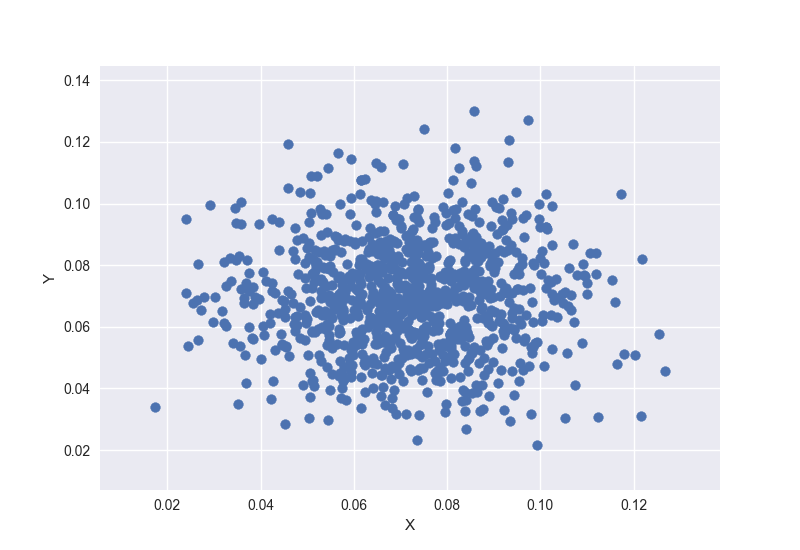
\includegraphics[scale=0.4]{initialization}
	\caption{Possible anchor node positions, between rovers (1000 iterations).}
	\label{fig:init}
\end{figure}

If each point in the figure is an agreed upon global reference point, then the graph suggests that our initialization algorithm is percise, but not entirely accurate. This is verified by Table~\ref{init_report}, where we can see that the mean of the distribution lies at roughly at (0.2, -0.01), which is approximately 20cm off of our goal reference point. This is close to our goal origin of (0,0), but while manuevering unique environments, confidence in current agent position is imperitive to accomplishing group tasks, thus this offset may present issues with complex algorithms. On the contrary, the low standard deviation of (0.0178, 0.01783), for $x$ and $y$ respectively, suggests that colaboratively each agent is finding the same common global point of reference between them, with minimal and excusivable error.

\begin{table}
	\centering
	\begin{tabular} {|| c | c | c ||}
		\hline 
		\multicolumn{3}{|| c ||}{\textbf{Classification Report}} \\
		\hline \hline
		& X & Y \\
		\hline
		Count & 1000 & 1000 \\
		Mean & 0.201831 & -0.014522 \\
		Std & 0.017800 & 0.017833 \\
		Min & 0.144812  & -0.065531 \\
		25\% & 0.190542 & -0.026514 \\
		50\% & 0.202951 & -0.014718 \\
		75\% & 0.213567 & -0.002392 \\
		Max & 0.257954 & 0.044440 \\
		\hline 
	\end{tabular}
	\caption{Classification report of the our Anchor Initialization algorithm over 1000 iterations.}
	\label{init_report}
\end{table}


Although, when working with non-static systems, small errors begin to expontentially grow and destroy the integrity of multi-agent control algorithms. To account for this we devised a 
Modeled below is graph of the localization of a single rover. The ideal path can be seen in black, originating at the origin (0,0) and traversing to point (1,3). 

\begin{figure} 
	\centering
	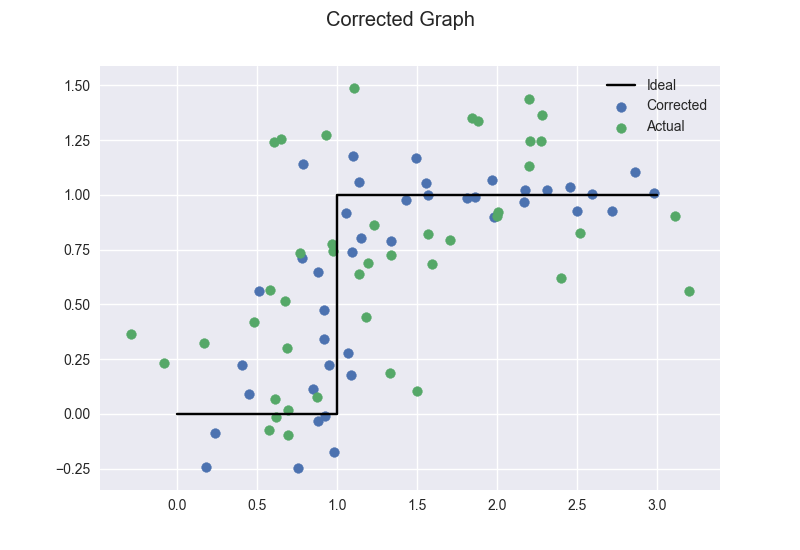
\includegraphics[scale=0.5]{localization}
	\caption{Dynamics localization as rover travels from (0,0) to (3,1).}
	\label{fig:dynamic}
\end{figure}


\begin{itemize}
	\item Mean Square Error = 0.0067 
	\item $R^2$ Regression Score = 0.964 
\end{itemize}


